\newlength{\mapcircle}

\setlength{\mapcircle}{.32\textwidth}

\newcommand\solarSystem{

  \centering

  \vspace{1\mapcircle}

  \begin{tikzpicture}[thick,remember picture,overlay]

    \draw[\pageSideColor,dotted,opacity=0.2] (0,0) circle(\mapcircle);

    \setcounter{track}{0}
    \foreach \x in {0,60,120,-60,-120,180} {
      \stepcounter{track}
      \path[fill,draw] (\x:\mapcircle) circle(0.5pt) {};
      \draw[\pageSideColor] (0,0) node{\Large 8};
      \draw[\pageSideColor] (\x:\mapcircle+2em) node{\Large\arabic{track}};
              }
  \end{tikzpicture}

  \vspace{\mapcircle}

}

\newcommand\encRef[1]{%
  \nameref{#1} (\autopageref{#1})%
}

\newcommand{\moralechart}{
  \begin{nametable}{Morale Chart}
    \textbf{Bonus} & \textbf{Situation} \\\hline

    +4 & Monsters outnumber characters 3:1. \\

    +2 & Monsters outnumber characters 2:1. \\

    +2 & Character's top Strength Bonus is lower than the monster's.  \\

    +2 & Monster is desperate or hungry.  \\

    -2 & Character's top Strength Bonus is higher than the monster's.  \\

    -2 & Characters outnumber the monsters. \\

    -2 & Monster is wounded. \\

    -1 & Characters have displayed awesome magical abilities. \\

      \end{nametable}
}

\newcommand\foragingChart{
  \begin{nametable}[c|p{.4\textwidth}|L|L]{Foraging}

    \textbf{Roll} & \textbf{Place} & \textbf{Prize 1} & \textbf{Prize 2}\\\hline

    \dicef{1} &
      Under a hidden floorboard -- broken patches show something underneath &
      \lootJewellery &
      \lootMagic \\

    \dicef{2} &
      Hidden room, behind an old bookcase &
      \lootJewellery &
      \lootJewellery, and \lootBig \\

    \dicef{3} &
      In empty home, inside a dark and empty doorway &
      \lootJewellery, and \lootJewellery &
      \lootJewellery, and \lootBig \\

    \dicef{4} &
      Inside a largely preserved house.
      The family died peacefully, somehow\ldots &
      \lootMedium{} and, surprise, woodspy! (\autopageref{woodspy}) &
      \lootJewellery \\

    \dicef{5} &
      Behind a fully stone door, clearly used as a safe.
    Opening it requires Intelligence + Crafts (\gls{tn} 12 to do so quietly, otherwise, \gls{tn} 7) & \lootJewellery & \lootMagic  \\

    \dicef{6} &
      Lying under a pile of human bones &
      \lootBig &
      \lootMagic \\

  \end{nametable}
}

\newcommand\encSummary{

  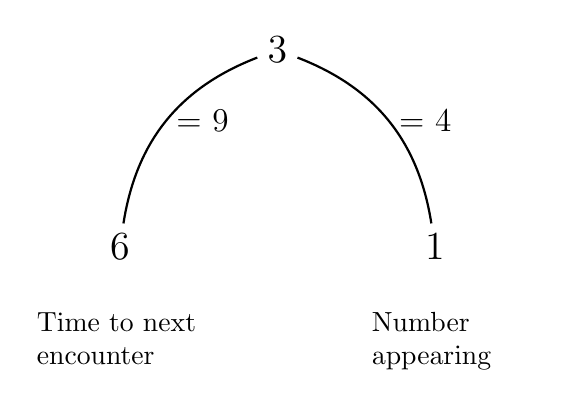
\begin{tikzpicture}[thick]

  \node (A) at (0,0){\Large\dicef{6}};

  \node (B) at (4,0){\Large\dicef{1}};

  \node (C) at (2,2.5){\Large\dicef{3}};

  \draw[\pageSideColor] (A) to[bend left] node[right]{\large\outline{= 9}}(C);

  \draw[\pageSideColor] (C) to[bend left] node[right,align=center]{\large\outline{= 4}}(B);

  %\draw (B) to[bend left]node[below]{\outline{7}} (A);

  \draw (A)+(0,-2em) node[below,text width=6em]{Time to next encounter};

  \draw (B.east)+(0,-2em) node[below,text width=6em]{Number \\ appearing};

  \end{tikzpicture}

}

\newcommand\cityRelations{

  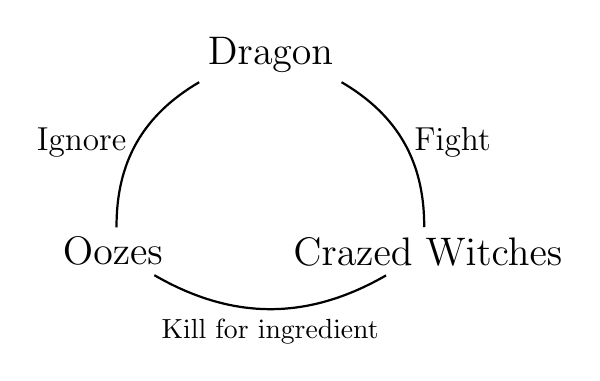
\begin{tikzpicture}[thick]

  \node (A) at (0,0){\Large Oozes};

  \node (B) at (4,0){\Large Crazed Witches};

  \node (C) at (2,2.5){\Large Dragon};

  \draw[\pageSideColor] (A) to[bend left] node[left]{\large Ignore}(C);

  \draw[\pageSideColor] (C) to[bend left] node[right]{\large Fight}(B);

  \draw[\pageSideColor] (B) to[bend left] node[below]{Kill for \Glspl{ingredient}} (A);

  \end{tikzpicture}
}

\newcommand\showBandits{
  \item
  \setcounter{gold}{\value{diceNo}}
  \multiply\value{gold} by 2
  \addtocounter{gold}{4}
  \arabic{gold} \ifodd\value{diceNo}
    Brigands
  \else
    Bandits
  \fi
}

\newcommand\encBandits{
  \begin{multicols}{2}
  \begin{dlist}
    \showBandits
    \showBandits
    \showBandits
    \showBandits
    \showBandits
    \showBandits
  \end{dlist}
  \end{multicols}
}

\newcommand\encTraders{
  \label{traderWares}
  \begin{multicols}{2}
  \begin{dlist}
    \item
    Fresh fruits (\arabic{r2}0~\glspl{cp} per day's worth)
    \randomdozen
    \item
    Bows (\arabic{r12}~\glspl{sp})
    and arrows (\arabic{r12}0~\glspl{cp})
    \randomdozen
    \item
    Torch pitch for (\arabic{r12}~\glspl{cp} per hour's worth)
    \randomdozen
    \item
    Salted meats (\arabic{r12}~\glspl{cp} per day's worth)
    \randomdozen
    \item
    Rope (\arabic{r12}0~\glspl{cp})
    \randomdozen
    \item
    Caged beast (use the creature from the encounter number)
  \end{dlist}
  \end{multicols}
}

\newcommand\encSight{%
  \ifcase\value{track}\relax%
  \or%
    Hibernating \encRef{chitincrawler}
  \or%
    Deer
  \or%
    \encRef{auroch}
  \or%
    \encRef{boar}
  \or%
    \encRef{mage_oak}
  \or%
    \encRef{uproot}
  \or%
    \encRef{bedleaves}
  \or%
    \encRef{marching_mushroom}
  \else%
    \encRef{seekmist}
  \fi%
  \stepcounter{track}%
}

\newcommand\trackMonth{%
  \ifcase\value{season}\or%
    January\or February\or March\or April\or May\or June\or%
    July\or August\or September\or October\or November\else December\fi%
}

\newcommand\showSeasonLine[1]{
  \setcounter{season}{#1}
  \trackMonth &
  \textbf{\showSeason} &
  \setTemperature
  \showTemperature &
  \showAstroEvents
  \\
}

\newcommand\encMonsters{
  \setcounter{enc}{1}
  \begin{boxtable}[cccL]
    \textbf{Cold} & \textbf{Mild} & \textbf{Hot}  & \textbf{Encounter} \\
    \hline
    \dicef{1} &           &           & \encMons                       \\
    \dicef{2} &           &           & \encMons                       \\
    \dicef{3} & \dicef{1} &           & \encMons                       \\
    \dicef{4} & \dicef{2} & \dicef{1} & \encMons                       \\
    \dicef{5} & \dicef{3} & \dicef{2} & \encMons                       \\
    \dicef{6} & \dicef{4} & \dicef{3} & \encMons                       \\
              & \dicef{5} & \dicef{4} & \encMons                       \\
              & \dicef{6} & \dicef{5} & \encMons                       \\
              &           & \dicef{6} & \encMons                       \\

  \end{boxtable}
}

\newcommand\stepDown[1]{
  \ifnum\value{#1}>1
    \addtocounter{#1}{-1}
    \ifnum\value{#1}<13
        \arabic{#1}
    \fi
  \fi
}

\newcommand\encLine{
  \stepDown{diceNo} & \stepDown{diceNo2} & \stepDown{enc} & 
}

\newenvironment{encChart}[1]%
  {
    \setcounter{diceNo}{13}
    \setcounter{diceNo2}{15}
    \setcounter{enc}{17}

    \rowcolors{2}{}{gray!10}
    \vspace{2em}
    \tabularx{\linewidth}{c|c|c|L}
      \hline
      \hline
      \textbf{Warm} & \textbf{Mild} & \textbf{Cold} & \textbf{#1} \\
      \hline
  }%
  {
      \hline
    \endtabularx
    \vspace{2em}
  }%

\newcommand\bigWeatherList{
  \ifcase\value{enc}\or%
    Cold snap
  \or%
    Hail
  \or%
    Snow
  \or%
    Biting winds (4 \glspl{mp})
  \or%
    Mild breeze
  \or%
    Dead calm (2 \glspl{mp})
  \or%
    Mist
  \or%
    Overcast sky
  \or%
    Brewing storm
  \or%
    Lightning (4 \glspl{mp})
  \or%
    Thunder
  \or%
    Clear skies
  \or%
    Light showers
  \or%
    Hurricane (4 \glspl{mp})
  \or%
    Heatwave (2 \glspl{mp})
  \or%
    Floods
  \else%
    Error
  \fi
}

\newcommand\bigBeastList{
  \ifcase\value{enc}\or%
    Roaming Ghast
  \or%
    $1D6$ Wandering Ghouls
  \or%
    Dryad
  \or%
    $1D6\times 2$ Elves on a quest
  \or%
    $1D6\times 3$ Deer
  \or%
    $1D6\times 20$ Aurochs
  \or%
    Warthog
  \or%
    Bear
  \or%
    $1D6+6$ Wolves
  \or%
    $1D3$ Griffins
  \or%
    Woodspy
  \or%
    Mouthdigger
  \or%
    Chitincrawler
  \or%
    Basilisk
  \or%
    Swarming stirges
  \or%
    Umber Hulk
  \else%
    Error! \LaTeX\ has broken, the beasts are loose!
  \fi%
}

\newcommand\encMountains{
  \ifcase\value{enc}\or%
    Roaming Ghast
  \or%
    $1D6$ Wandering Ghouls
  \or%
    Dryad
  \or%
    $1D3\times 2$ Elves back from a quest
  \or%
    $1D6\times 3$ Goats
  \or%
    \relax
  \or%
    \relax
  \or%
    \relax
  \or%
    \relax
  \or%
    $1D3$ Griffins
  \or%
    \relax
  \or%
    \relax
  \or%
    \relax
  \or%
    Umber Hulk
  \or%
    Bear
  \or%
    Swarming stirges
  \else%
    Error! \LaTeX\ has broken, the beasts are loose!
  \fi%
}

\newcommand\encLakeside{
  \ifcase\value{enc}\or%
    \relax
  \or%
    \relax
  \or%
    Dryad
  \or%
    $1D6\times 2$ Elves lounging
  \or%
    $1D6\times 3$ Deer
  \or%
    $1D6\times 20$ Aurochs
  \or%
    Warthog
  \or%
    Bear
  \or%
    $1D3$ Griffins
  \or%
    Woodspy
  \or%
    \relax
  \or%
    $1D6+6$ Wolves
  \or%
    Chitincrawler
  \or%
    Basilisk
  \or%
    Swarming stirges
  \or%
    \relax
  \else%
    Error! \LaTeX\ has broken, the beasts are loose!
  \fi%
}


%%%%% Full Encounters %%%%%

\newcommand\encTownEvents{
  \index{Towns!Events}
  \index{Events!Towns}
  \setcounter{diceNo2}{6}
  \setcounter{diceNo}{6}
  \begin{wideTable}[c|c|LL]{Town Events}
  \hline
  \textbf{Day} & \textbf{Night} & \textbf{Market} & \textbf{Tavern} \\
  \hline
  \Large\dicef{6} & &
              A doula offers to sell \glspl{boon} for 3 \glspl{sp} each. &
              Dead: nobody there.
              \\
  \Large\dicef{5} & &
              A doula wants to purchase \glspl{ingredient}, for 50 \glspl{cp} each. &
              Mostly dead: a single barman, and an alcoholic.
              \\
  \Large\dicef{4} & \Large\dicef{6} &
              A trader stands outside a workshop, screaming that a cart fixer produces shoddy goods (`I almost died, out in the forest, when a wheel came off').  Moments later, the cart fixer attacks. &
              Two drinkers and two traders, discussing local prices.
              \\
  \Large\dicef{3} & \Large\dicef{5} &
              The \gls{templeOfCuriosity} have a famed Storyteller visiting, and everyone wants to know where dragons come from, in his latest tale of mystery and magic. &
              A dozen patrons, complaining about local crime, and hoping to see the \gls{court}.
              \\
  \Large\dicef{2} & \Large\dicef{4} &
              The workers at the bakers guild are rebelling, and have staged a walkout.  Within a day, the Guild leaders will slip poison into the drinks of the organizers. &
              Myriad customers, all in for a quick drink. The bar empties soon after.
              \\
  \Large\dicef{1} & \Large\dicef{3} & A merchant is selling basilisk flesh which he found on the side of the road.  When guards ask if he took the basilisk recently killed by the \gls{guard}, he says `no', and that his cousin sold it to him. &
              A slap-fight breaks out between two \glspl{seeker}, as one won't tell the other the answer to a riddle.
  \\
            & \Large\dicef{2} &
                        A shady fence hangs around the market, whistling a happy tune.  He left all his goods in a nearby, seedy tavern's basement. &
                        Nine confused patrons sit in a corner, surrounded by a wedding party of hundreds.
                        \\
            & \Large\dicef{1} &
                        Four thugs, waiting to rob anyone who looks weak. &
                        The barkeep is raving at people to fetch him \pgls{doula} for his illness (Mindflash Syndrome, \autopageref{Mindflash Syndrome}), but none will come since he insulted \pgls{doula} last year.
                        \\
  \hline
  \end{wideTable}
}

\newcommand\brochEvents{
  \index{Events!\Glspl{broch}}
  \begin{dlist}
  \item
  Help!
  I can't nail this yurt down properly.
  If it's not secured, something might eat the horses (they can't go inside).
  \item
  The \gls{broch}'s \gls{jotter} has some emergency-tasks, but the \gls{broch} has a dozen \gls{guard} archers, so we'll manage.

  Roll for two missions (\vpageref{ngMissions}); if any \gls{pc} has a higher rank than `Archer', then they can select which mission to take, and which to give to the Archers.
  Otherwise, the \glspl{pc} receive the mission with the highest number.
  \item
  A dozen \glspl{guard} archers sleep here alread, with \pgls{jotter} upstairs.
  \item
  Two griffins rest on top of the \gls{broch}, and nobody inside knows what to do about them.
  They're out of line of site, and very high up, so arrows won't hit anything.
  \item
  Dreameater moss covers the \gls{broch}'s sides, and someone's already had a nightmare.
  Nobody wants to sleep in this place, but nobody wants to scrape moss from the tall walls either.
  \item
  The \gls{broch} needs bricks (large creatures and storms dislodged a few).
  Deliveries should arrive soon, but in the meantime, someone needs to keep an eye on the roof, and make sure nothing crawls inside.
  \end{dlist}
}

\newcommand\bothyEvents{
  \index{Events!\Glspl{bothy}}
  \begin{dlist}
  \item
  All full!
  Seriously, we have a dozen horses and two dozen people in here.
  You're the \gls{guard} -- sleep outside!
  \item
  Nice and comfy \gls{bothy}, with two piles of logs.
  Only one of them is a woodspy\ldots
  \item
  Two \gls{guard} deserters have camped here the last week, begging food from passing traders.
  They have ignored the last orders received from \pgls{jotter} (roll \vpageref{ngMissions}) and will soon turn to banditry.
  Both have the rank of `Fodder', and will lie about their situation, saying \pgls{jotter} asked them to guard the \gls{bothy}.
  \item
  This \gls{bothy} lies empty.
  The roof could do with some repairs, and the door's seen better days.
  \item
  The last group never left any fire wood.
  They took the firewood axe as well.
  \item
  A few traders have settled in.
  They will spend the night trying to sell their wares to the troupe (find their wares \vpageref{traderWares}).
  \end{dlist}
}

\newcommand\encVillageEvent{
  \begin{dlist}
  \stepcounter{dlist}
    \ifodd\value{r4}
      \item
      A child steals from one of the characters.
      \item
      A local archer shot down a griffin. It now sits in the central square, on a spit-roast.
      \item
      Children have spotted a woodspy, camouflaging itself into a tree.
      A dozen have gathered to throw rocks at it from a `safe' distance.
    \else
      \item
      A scout has destroyed a chitincrawler's nest and found an interesting item.
      \lootMagic.
      \item
      Basilisk-stench assaults the troupe's faces.
      Someone sunk a lucky arrow into a basilisk's eye a month ago, but without the proper equipment, the \gls{village} could only pull a little meat off it before the corpse spoiled.
      Farmers pulled chunks off for a while, but traders refuse to help take it away with them.
      At present, the entire \gls{village} has just resigned itself to stinking until the problem goes away itself.
      \item
      The villagers hold a funeral for a fallen soldier. Everyone is drunk.
    \fi
    \item
    \ifodd\value{r3}
      Villagers are constructing a wooden cage to safely take water from the river, so woodspies do not drown them, and eat them.
    \else
      Villagers gather to burn away or cut down all the foliage and trees they can, making space for their archers to see.
    \fi
    \item
    A few mouthdiggers have burrowed under the \gls{village}.
    You can hear them at night.
    The villagers discuss plans to root them out, but nobody has anything solid.
    \item
    Rumours of local oddity (see \autopageref{mapOddities}).
    \item
    A boy wants to join the characters band, his family disapproves but he will try everything he can.
    \item
    A guard has saved $1D6 \times 30$~\gls{sp}, and now hides in the \gls{village}, having abandoned his duties.
    \item
    A griffin has picked up a child, and flown into the forest.
    A dozen farmers prepare to go after it, but they move too slowly.
    \roll{Speed}{Athletics}, \tn[11] to get to the child on time.
    \item
    A troupe of \gls{village} elders, armed with spears, return to report they have seen the local fiend in the forest (from \autopageref{mapFiends}).
    \item
    A wall has broken, and $2D6$ pigs run loose in the forest.
  \end{dlist}
}

\newcommand\encVillageFeatures{
  \begin{dlist}
  \stepcounter{dlist}
    \item
    Verdant \nameref{screeching_moss} grows along the old, outer walls (find it \vpageref{screeching_moss}).
    \item
    Four long, wooden entrances sit around the perimeter.
    Each one ends in a metal gate, showing people inside, and each stretch of wood is littered with murder-holes, ready for archers and spearmen to slay anything which approaches the gate.
    \item
    A massive moat, wider than anyone could hope to jump, flows round the outskirts. 
    \item
    Long, thin, copper spikes crown the outer wall.
    Most are fully green, but some chromatic, shining patches show where a creature's body has fallen to them.
    \item
    Tiny wire fences surround every field around the outskirts.
    The bells and chimes make a gentle sound in the wind, and a far louder noise is anything mounts those fences.
    \item
    The fields are covered in meat-on-sticks, and the meats are covered in poison.
    Eating the poison should inflict 8 \glspl{fatigue} to local predators.
    Dead rats and foxes litter the area, indicating that the plan has some problems.
    \item
    Bear traps surround the perimeter, hidden by grass, bush, and cabbages.
    The locals know where every single one lies.
    Spot them with \roll{Wits}{Vigilance} (\tn[10]), with $1D6$ Damage for failure.
    \item
    $1D3$ tripple-bows sit along the wall (giant crossbows on wheels).
    They inflict $3D6$ Damage, but inflict a -2 penalty to aim.
    \item
    A large motte shows \pgls{warden} lives here.
    \item
    A little house, built into the ground, suggests a doula lives here.
    \item
    A patch of \nameref{uproot} grows just beyond the treeline (\autopageref{uproot}).
  \end{dlist}
}

\newcommand\ngMissions{
  \label{ngMissions}
  \begin{enumerate}
    \item
    The \gls{jotter} says to
      \begin{dlist}
        \item
        clean out the shit-pits; his first, his horse's second, then everyone else's.
        \item
        shine his armour.
        \item
        take his wine delivery up to his room, at the top of the \gls{broch}.
        \item
        clean the \gls{broch}, top to bottom.
        \item
        give a complete recount of the area you come from.
        They need the information for `data related purposes'.
        \item
        check the perimiter -- just run round everywhere that's not forest.
      \end{dlist}
    \item
    Help \pgls{village}
    \begin{dlist}
      \item
      by watching over its sheep.
      Something nasty has taken ten from inside a locked bar, and nobody knows how.
      \item
      by widening their road.
      Spend the next week going along the road, cutting, burning, and pushing back the forest.
      The \gls{village} will feed you.
      \item
      \ifnum\value{temperature}=0
        deal with its undead problem, but \emph{don't} come back here a dead, moaning failure, alright!?.
      \else
        deal with its basilisk problem.
        Bonus points for finding the nest.
      \fi
      \item
      clear the perrimiter -- they need someone to raise and chop all around the edges.
      \item
      with a particularly large griffin.
      They say it picked up a pregnant ewe!
      \item
      to defeat the local brigands.
      If the brigands find out about the \glspl{pc}, they will simply leave for a season.
    \end{dlist}
    \item
    Help transport a
    \begin{multicols}{2}
    \begin{dlist}
      \item
      child
      \item
      convict
      \item
      guild leader
      \item
      wounded ranger
      \item
      magical item
      \item
      secret document
    \end{dlist}
    \end{multicols}
    \ldots to the next town.
    \item
    A Night Rider needs you to
    \label{riderMissions}
    \begin{dlist}
      \item
      lay these three traps around a nearby \gls{village}.
      They weight a tonne, so take these six donkeys and just try to work something out.
      \item
      deliver a message to a local fiend.
      You do not have to approach them, but you \emph{do} need evidence that they received the message.
      \label{fiendLetter}
      \item
      track down and kill a team of local bandits, out beyond the \gls{edge}.
      \item
      tell a distant \gls{village} to resume paying their taxes to their \gls{warden}, and start causing trouble if they refuse.
      \label{taxesMission}
      \item
      clear a road blocked by some creature (use the highest possible monster roll for the place and season).
      \item
      hunt down a half-elven sorcerer who leads a crew of bandits.
    \end{dlist}
    \item
    A travelling tradesman wants you to
      \begin{dlist}
        \item
        come guard his caravan on a journey to the next town.
        He'll pay you 30~\glspl{sp}.
        \item
        take this shortsword -- it should keep you safe.
        \item
        \ifodd\value{r4b}
          tell him about what the \gls{guard} are up to.
          He will join you on the road and pay 5 \glspl{sp} per person for the `news'.
        \else
          join her going to the next town, and vouch that the bag of 300 \glspl{sp} belongs to the \gls{guard} and not her, so she doesn't have to pay a tax on it.
        \fi
        \item
        tell her about any interesting things you might have found on the road\ldots
        anything you maybe haven't reported to the \gls{jotter}\ldots
        maybe something you need help getting rid of\ldots?
        \item
        help deliver something to a local fiend.
        The tradesman has just what it wants
      (as per \autopageref{fiendDesires}).
        She can pay a total of 60~\glspl{sp}.
        \item
        break a friend out of jail in a nearby town.
        He had no idea those items were stolen!
      \end{dlist}
    Tell nobody -- you could get in a lot of trouble for moonlighting
    (re-roll to find your orders).
  \item
  Seek out the
    \begin{dlist}
      \item
      \gls{guard} deserter, and prosecute them in the local \gls{court}.
      \item
      local oddity and find out what you can
      (see \nameref{mapOddities}, \autopageref{mapOddities}).
      \item
      elven fence, who sells stolen items to traders from far-away lands.
      \item
      native speaker of Gnomish, because someone needs a book translated.
      \item
      doula, famed for her healing abilities, to help the local \gls{warden}.
      \item
      local fiend, and find out what it wants
      (as per `\nameref{fiendDesires}', \autopageref{fiendDesires}).
    \end{dlist}
  \item
  Capture a
    \begin{dlist}
      \item
      bard, known for spreading completely unverified rumours about the \glspl{warden}.
      \item
      witch, who keeps casting strange and deadly enchantments on local plants.
      \item
      place where mana wells up from the ground. It lies somewhere in the forest, or so the bards sing.
      \item
      creature for the arena; the \glspl{warden} want to see some good sport.
      \item
      ray of full moonlight.
      The doula need it for something, but won't explain what they mean.
      \item
      thief in the act. He robs \glspl{warden} at night, but nobody has seen his face.
    \end{dlist}
  \item
  A builder needs you to travel beyond the \gls{edge} and
    \begin{dlist}
    \item
    find where those goblins come from.
    \item
    confirm what you can about this map -- it makes some strange claims.
    \item
    bring back a feast of basilisk eggs -- the \gls{warden} wants to impress a lady.
    \item
    recover the golden wand from the lost city.
    We hear it lies there, but if we heard wrong, return with evidence that there is no lost city there.
    \item
    confirm the doula's claims about the great site for starting a new \gls{village}.
    \item
    deliver this message to the local elves, or gnomes, or whatever they are.
    \end{dlist}
  \item
  Take the day off -- you've earned it!
  \end{enumerate}
}

\newcommand\randomDisease{
  \begin{dlist}
    \item
    Breathrot
    \item
    Corpse Hands
    \item
    Mindflash Syndrome
    \item
    Guardbane
    \item
    Spychoke
    \item
    Torpid Flesh
  \end{dlist}
}

\newcommand\missionComplications{
  \label{missionComplications}
  \begin{enumerate}
    \item
    The \gls{jotter} has assigned a Cutter to stand watch over everything you do.
    They won't help, they only make sardonic comments.
    \item
    Take this Wanderer from the \gls{paperGuild} with you to chronicle the mission.%
    \footnote{See \autopageref{knowledgeWanderer} for Wanderers.}
    And \emph{don't} let him get hurt.
    \item
    There are two of them!%
      \footnote{If the troupe need to transport a wounded ranger, they hear about another wounded ranger en route, and have to rescue the other as well (after finding them).
      If the troupe need to find a doula, then the doula tells them they first have to help find her sister.}
    \item
    Roll twice more!
    \item
    The troupe leader has developed a nasty disease (see \autopageref{diseases}).
    \randomDisease
    \item
    Rival \glspl{guard} work on a related mission.
    Roll the second $D6$ again, to find their quarry.
    Both items are related.%
    \footnote{
      For example, if you roll a \ref{riderMissions} then \ref{fiendLetter}, the \glspl{pc} would have to deliver a letter to a fiend.
      If the rivals rolled a \ref{taxesMission}, they would have to threaten a \gls{village} into paying its taxes, and these two missions would interfere with each other somehow.

      Perhaps both missions involve targets who travel together, or perhaps one mission's success leads to the other's failure.
    }
    \item
    A distant \gls{warden} hopes for their failure, and has sent his men to stop them.
    \item
    A nearby fiend does not want the mission to succeed.
    \item
    The \gls{templeOfPoison}%
    \footnote{See \autopageref{god:Poison}.}
    has a vested interest in the mission failing, and will influence all the groups they can to stop the troupe succeeding.
    If the troupe have an encounter with an intelligent creature (such as a bandit or trader) there is a 50\% chance they work as a spy for the \gls{templeOfPoison}.
  \end{enumerate}
}

\newcommand\newBeast[4][\A]{
  \subsubsection[#2 (#1): #4.]{#1~#2}
  \label{#3}
  \index{#2 (#1)}
}

\newcommand\exampleGoblinEnc{
  \setcounter{enc}{15}
  \setcounter{diceNo}{13}
  \vspace{2em}
  \rowcolors{2}{}{gray!10}
  \noindent
  \begin{boxtable}[c|L]
    \hline
    \hline
    \textbf{Roll} & \textbf{Inner Hamlets} \\
    \hline
    \Repeat{5}{
      \addtocounter{diceNo}{-1}
      \addtocounter{enc}{-1}
      \arabic{diceNo} & \bigBeastList \\
    }
    \hline
    \addtocounter{diceNo}{-1}
    \addtocounter{enc}{-1}
    \arabic{diceNo} & \ifodd\value{enc}Brigands!\else Bandits\fi \\
    \hline
    \Repeat{3}{
      \addtocounter{diceNo}{-1}
      \addtocounter{enc}{-1}
      \arabic{diceNo} & \arabic{diceNo} wagons \\
    }
    \hline
    \Repeat{3}{
      \addtocounter{diceNo}{-1}
      \addtocounter{enc}{-1}
      \arabic{diceNo} & \multiply\value{diceNo} by 4 \arabic{diceNo} goblins! \\
    }
    \hline
  \end{boxtable}
}

\newcommand\hitLocation{
  \begin{boxtable}[XXXX]
    \textbf{Damage} & \textbf{Location} & \textbf{Slash} & \textbf{Bash} \\
    \hline
    \dicef{1} & ear & cut & bruised \\
    \dicef{2} & cheek & slashed & bashed \\
    \dicef{3} & belly & spliced & smashed \\
    \dicef{4} & ribs & pierced & shattered \\
    \dicef{5} & arm & mutilated & crippled \\
    \dicef{6} & thigh & gashed open & cracked \\
    \dicef{7} & jaw & thwacked & chiseled \\
    \dicef{8} & shin & segmented & splintered \\
    \dicef{9} & skull & bisected & demolished \\
    \dicef{10} & heart & opened & interrupted \\
  \end{boxtable}
  }

\newcommand\showEnc[1][beasts]{%
  \needspace{3em}
  \begin{center}
  \gls{#1}\qquad\textbf{Encounters}\qquad\gls{#1}
  \end{center}
}
